\documentclass{beamer}
% \mode<presentation>
\setbeamertemplate{navigation symbols}{}
\let\tempone\itemize
\let\temptwo\enditemize
\newcommand{\din}{{d_{\mathrm{in}}}}
\newcommand{\dhid}{{d_{\mathrm{hid}}}}
\newcommand{\dwin}{{d_{\mathrm{win}}}}
\newcommand{\dout}{{d_{\mathrm{out}}}}
\newcommand{\demb}{{d_{\mathrm{emb}}}}

\renewenvironment{itemize}{\tempone\addtolength{\itemsep}{0.5\baselineskip}}{\temptwo}
% \usepackage{beamerthemeshadow}
\usepackage{tikz}
\usepackage{bbm}
\usepackage{hyperref}
\usepackage{natbib}
\usepackage{pgffor}
\usepackage{booktabs}
\usepackage{graphicx}
\usepackage{amssymb}
\usepackage{tabularx}
\usepackage{tikz,etoolbox}
\usepackage{tikz,amsmath,siunitx}
\usetikzlibrary{arrows,snakes,backgrounds,patterns,matrix,shapes,fit,calc,shadows,plotmarks}
\usepackage{tikz-qtree}
\newcommand{\softmax}{\mathrm{softmax}}
\usepackage[normalem]{ulem}
\newcommand\tst{% thick strike through  %% from http://tex.stackexchange.com/questions/134088/mis-alignment-of-columns-in-tabular-environment-when-using-ulem-and-beamer
  \bgroup%
  \markoverwith{\textcolor{red}{\rule[1.1ex]{1pt}{0.8pt}}}%
  \ULon%
}

\AtBeginSection[]
{
  \begin{frame}
  \frametitle{Contents}
  \tableofcontents[currentsection]
  \end{frame}
}

\usepackage{subcaption}
\usepackage[absolute,overlay]{textpos}
\usepackage{pgf}
\usepackage{latexsym}
\usepackage{amsfonts}
\usepackage{amssymb}
\usepackage{amsthm}
\usepackage{algorithm}
\usepackage{amsmath}
\usepackage{tabularx}
\usepackage{xcolor}
\usepackage[absolute,overlay]{textpos}
\usetikzlibrary{shapes,arrows,positioning,automata,positioning,spy,matrix,scopes,chains}
\newcommand{\digs}[2]{\hphantom{999}\llap{#1}\,+\,\hphantom{999}\llap{#2}}
\setbeamersize{text margin left=6mm}
\setbeamersize{text margin right=6mm}
\renewcommand{\insertnavigation}[1]{}
\setbeamertemplate{headline}{}
\setbeamertemplate{footline}{}
\usefonttheme{professionalfonts}
\setbeamercovered{transparent}
\mode<presentation>
\linespread{1.25}
\DeclareMathOperator{\Tr}{Tr} 

\usepackage{color}
\usepackage{multirow}
\usepackage{rotating}
\usepackage[all,dvips]{xy}
\usepackage{colortbl}
\usepackage{graphicx}
\usepackage{verbatim}
\usepackage{framed}
\usepackage{natbib}
\usepackage[labelformat=empty]{caption}
\newcommand{\air}{\vspace{0.25cm}}
\newcommand{\mair}{\vspace{-0.25cm}}

\setbeamertemplate{navigation symbols}{}%remove navigation symbols
\renewcommand{\rmdefault}{crm}
\newcommand{\lnbrack}{{\normalfont [}}
\newcommand{\rnbrack}{{\normalfont ]}\thinspace}
\newcommand{\lbbrack}{\textcolor{red}{\textbf{[}}}
\newcommand{\rbbrack}{\textcolor{red}{\textbf{]}}\thinspace}
\definecolor{vermillion}{RGB}{213,94,0}
\newcommand{\given}{\,|\,}
\definecolor{orange}{RGB}{230,159,0}
\definecolor{skyblue}{RGB}{86,180,233}
\definecolor{bluegreen}{RGB}{90,143,41}
% \definecolor{bluegreen}{RGB}{0,158,115}
\definecolor{myyellow}{RGB}{240,228,66} % i dunno if this is the same as standard yellow
\definecolor{myblue}{RGB}{0,114,178}
\definecolor{vermillion}{RGB}{213,94,0}
\definecolor{redpurple}{RGB}{204,121,167}
\definecolor{lightgrey}{RGB}{234,234,234}

\newcommand{\clust}{\ensuremath{\mathrm{clust}}}
\newcommand{\loc}{\ensuremath{\mathrm{loc}}}
\newcommand{\nicein}{\ensuremath{\,{\in}\,}}
\newcommand{\niceq}{\ensuremath{\,{=}\,}}
\newcommand{\uc}{\ensuremath{\mathrm{c}}}
\newcommand{\hc}{\boldh_{\uc}}
\newcommand{\cb}{\boldb_{\mathrm{\uc}}}
\newcommand{\cW}{\boldW_{\mathrm{\uc}}}
% \newcommand{\tanh}{\mathrm{tanh}}

\newcommand{\ha}{\boldh_{\ua}}
\newcommand{\hp}{\boldh_{\up}}

% \newcommand{\boldx}{\mathbf{x}}
\newcommand{\boldy}{\mathbf{y}}

% \newcommand{\hc}{\boldh_{\mathrm{c}}}


\def\kargmax{\operatornamewithlimits{K-arg\,max}}
%\DeclareMathOperator{\topK}{topK}
\def\topK{\operatornamewithlimits{topK}}
\DeclareMathOperator{\suk}{succ}
\newcommand{\longpfx}[1]{\ensuremath{w_1 \cdots w_{#1}}}
\newcommand{\longgoldpfx}[1]{\ensuremath{y_1 \cdots y_{#1}}}
\newcommand{\pfx}[1]{\ensuremath{w_{1:{#1}}}}
\newcommand{\goldpfx}[1]{\ensuremath{y_{1:{#1}}}}
\newcommand{\beampred}[2]{\ensuremath{\hat{y}_{1:{#1}}^{({#2})}}}
\newcommand{\boldx}{\mathbf{x}}

\usetikzlibrary{positioning}
% \setbeamerfont{alerted text}{series=\bfseries}
% \setbeamerfont{structure}{series=\bfseries}
% Needed for diakgrams.
\def\im#1#2{
  \node(#1) [scale=#2]{\pgfbox[center,top]{\pgfuseimage{#1}}
};}
% \input{pictures_header}


\title[Seq2seq]{CS 109b \\   LSTMs and Translation }


\author[Alexander Rush]{Alexander Rush  (@harvardnlp) \\  
% {\scriptsize  (with  Yoon Kim, Sam Wiseman, Hendrik Strobelt, Yuntian Deng, Allen Schmaltz) } \\
% \url{http://www.github.com/harvardnlp/seq2seq-talk/}
} 

% \institute[Harvard SEAS]{ \\
%   \begin{center}
%     
\includegraphics[width=1.3cm]{seas}
%   \end{center}

% }
\date{}
% \usetheme{Madrid}

\newcommand{\enc}{\mathrm{src}}
\newcommand{\xvec}{\mathbf{x}}
\newcommand{\yvec}{\mathbf{y}}
\newcommand{\wvec}{\mathbf{w}}
\newcommand{\cvec}{\mathbf{c}}
\newcommand{\zvec}{\mathbf{z}}
% \newcommand{\mcY}{\mathcal{Y}}
% \newcommand{\mcV}{\mathcal{V}}
\newcommand{\context}{\mathbf{w}_{\mathrm{c}}}
\newcommand{\embcontext}{\mathbf{\tilde{w}}_{\mathrm{c}}}
\newcommand{\inpcontext}{\mathbf{\tilde{x}}}
\newcommand{\start}{\mathbf{\tilde{y}}_{\mathrm{c0}}}
\newcommand{\End}{\mathrm{\texttt{</s>}}}

\newcommand{\Uvec}{\mathbf{U}}
\newcommand{\Evec}{\mathbf{E}}
\newcommand{\Gvec}{\mathbf{G}}
\newcommand{\Fvec}{\mathbf{F}}
\newcommand{\Pvec}{\mathbf{P}}
\newcommand{\pvec}{\mathbf{p}}
\newcommand{\Qvec}{\mathbf{Q}}
\newcommand{\Vvec}{\mathbf{V}}
\newcommand{\Wvec}{\mathbf{W}}
\newcommand{\hvec}{\mathbf{h}}
% \newcommand{\reals}{\mathbb{R}}

\newcommand{\Cite}[1]{}
\newcommand{\TT}[1]{{\footnotesize\tt{#1}}}
\newcommand{\boldw}{\boldsymbol{w}}
\newcommand{\boldu}{\boldsymbol{u}}
\newcommand{\boldv}{\boldsymbol{v}}
\newcommand{\boldb}{\mathbf{b}}
\newcommand{\boldW}{\mathbf{W}}
\newcommand{\boldh}{\boldsymbol{h}}
\newcommand{\boldg}{\boldsymbol{g}}
\newcommand{\ua}{\ensuremath{\mathrm{a}}}
\newcommand{\up}{\ensuremath{\mathrm{p}}}
%\newcommand{\bphi}{\ensuremath{\mathbf{\phi}}}
\newcommand{\bphi}{\boldsymbol{\phi}}
\newcommand{\btheta}{\boldsymbol{\theta}}
\newcommand{\mcY}{\mathcal{Y}}
\newcommand{\mcX}{\mathcal{X}}
\newcommand{\mcC}{\mathcal{C}}
\newcommand{\mcA}{\mathcal{A}}
\newcommand{\mcV}{\mathcal{V}}
\newcommand{\trans}{\ensuremath{\mathsf{T}}}
\def\argmin{\operatornamewithlimits{arg\,min}}
\def\argmax{\operatornamewithlimits{arg\,max}}
\newcommand{\reals}{\ensuremath{\mathbb{R}}}

\newcommand{\aphi}{\boldsymbol{\phi}_{\mathrm{a}}}
\newcommand{\pwphi}{\boldsymbol{\phi}_{\mathrm{p}}}
\newcommand{\squigaphi}{\widetilde{\boldsymbol{\phi}}_{\mathrm{a}}}
\newcommand{\squigpwphi}{\widetilde{\boldsymbol{\phi}}_{\mathrm{p}}}

\newcommand{\aW}{\boldW_{\mathrm{\ua}}}
\newcommand{\pW}{\boldW_{\mathrm{\up}}}

\newcommand{\ab}{\boldb_{\mathrm{\ua}}}
\newcommand{\pb}{\boldb_{\mathrm{\up}}}

\newcommand{\Da}{d_{\mathrm{a}}}
\newcommand{\Dp}{d_{\mathrm{p}}}

% \newcommand{\ha}{\boldh_{\ua}}
% \newcommand{\hp}{\boldh_{\up}}

\newcommand{\ourmodel}{This work}
\newcommand{\zro}{{\color{white}0}}


\def\argmax{\operatornamewithlimits{arg\,max}}
\def\kargmax{\operatornamewithlimits{K-arg\,max}}

\begin{document}

\begin{frame}
  \titlepage
\end{frame}

\begin{frame}
  \structure{Where we are going.}
  \begin{center}
    \includegraphics[width=12cm]{nmtexamples}
  \end{center}

\end{frame}

\begin{frame}
  \begin{center}
    \alert{Last Class:} \\ Language Modeling, Embeddings, and RNNs
  \end{center}
  
  \textbf{Aim}:  model the probability of 
  \[ p(w_t | w_1, \ldots, w_{t-1}) \] 
  \air

  \textbf{Approach:} utilize a neural network to compute probabilities.
\end{frame}

\begin{frame}%{Deep Learning Toolbox}
  \begin{center}
    \alert{RNN For Language Modeling}
    \air 
  \end{center}
  \begin{center}
    \begin{tabular}{cclll}
      \structure{Embeddings} & & words &$\Rightarrow$& word vectors \\\\
      % \structure{Convolutions} &&  feature n-grams & $\Rightarrow$& dense features  \\\\

      \structure{RNNs} & & word vectors & $\Rightarrow$ & hidden states  \\\\
      \structure{Softmax} & & hidden states & $\Rightarrow$ & word prediction \\
    \end{tabular}
  \end{center}
\end{frame}


\begin{frame}{Words Embeddings}
  \begin{center}
    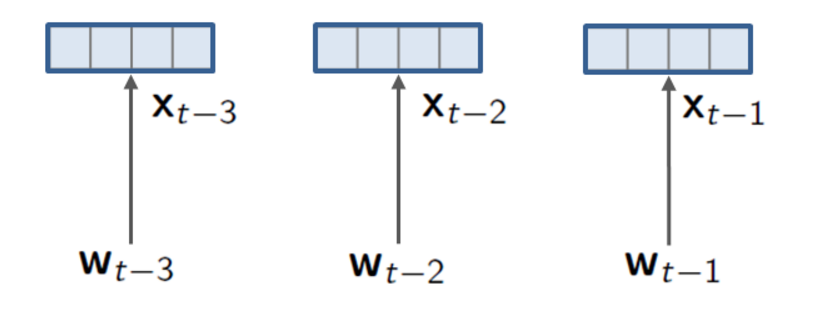
\includegraphics[width=7cm]{emb}
  \end{center}
  \begin{itemize}
  \item Map words to vector space, just as before. 
  \end{itemize}

\end{frame}

\begin{frame}
  \begin{center}
    \includegraphics[height=0.9\textheight]{graph}

    \href[pdfnewwindow=true]{http://harvardnlp.github.io/seq2seq-talk/web/wordvecs.html}{[Words Vectors]}
   \end{center}
\end{frame}

\begin{frame}{RNN}
  \begin{center}
    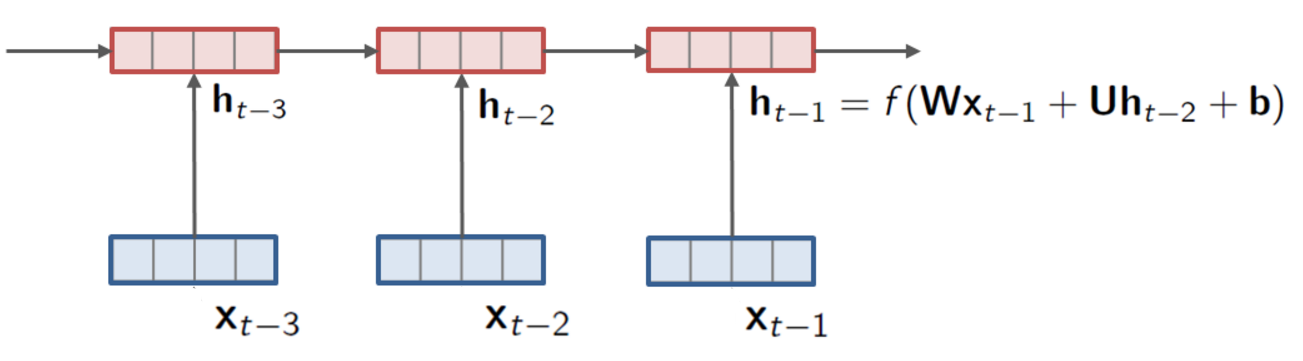
\includegraphics[width=11cm]{rnn}
  \end{center}  
  \begin{itemize}
  \item Apply recurrent neural network over vector space of words to create hidden states.
  \end{itemize}
\end{frame}




\begin{frame}{Softmax}
  \begin{center}

    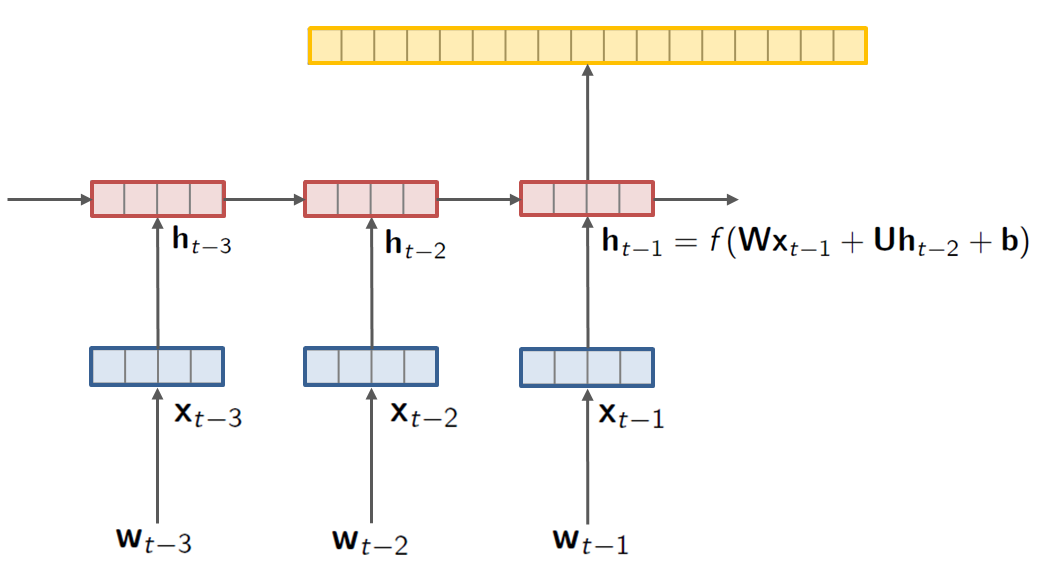
\includegraphics[width=0.8\textwidth]{rnnlm5}
  \end{center}
    
  \begin{itemize}
  \item Compute softmax over all possible next words to predict.
  \end{itemize}
  \[  p(w_t \given w_1, \ldots, w_{t-1}) = \sigma(\mathbf{W} \mathbf{h}_{t-1} + \mathbf{b})_w \] 

  % \[ p(w_{1:T} ) = \prod_{t} p(w_t | w_1, \ldots, w_{t-1}) \] 
    % \caption{Xu et al (2015)}  
\end{frame}

\section{LSTMs}

\begin{frame}{RNN Mathematically}


  Let $h_0 \gets 0$, 
  \[ h_1 \gets \textbf{RNN}(h_{0}, \boldx_1;\theta) \] 
  \[ h_2 \gets \textbf{RNN}(h_{1}, \boldx_2;\theta) \] 
  \[ h_3 \gets \textbf{RNN}(h_{2}, \boldx_3;\theta) \] 
  \centerline{$\vdots$}
  \[ h_n \gets \textbf{RNN}(h_{n-1}, \boldx_n;\theta) \] 
  
  Where RNN is a neural network layer with the same weights $\theta$ applied 
  at each time step, for instance: 
  
  \[ \textbf{RNN}(h, \boldx) = \tanh(\boldW h + \mathbf{U} \boldx) \] 
\end{frame}


\begin{frame}
  What types of relationships  might  the network to learn?

  \begin{eqnarray*}
  \textbf{ExpAvg}(h, \boldx) &=& \tanh(\alpha\boldx + (1-\alpha) h) \\
   \textbf{LastWord}(h, \boldx) &=& \tanh(\boldx) \\
   \textbf{ConcatLast2}(h, \boldx) &=& \tanh([\textbf{U} \boldx, \boldW \boldh])\\
 \end{eqnarray*}
  
  (Formally, a non-linear IIR transformation.)
\end{frame}

\begin{frame}{Issues with Basic RNN}

  \begin{center}
    \Tree [ .$h_n$ [ .$\ldots$ [ .$h_3$ [ .$h_2$ [ .$h_1$ $h_0$ $\boldx_1$ ]
    $\boldx_2$ ] $\boldx_3$ ] $\ldots$ ] $\boldx_n$ ]
  \end{center}

  Very deep network. Can be hundreds of layers of non-linear transformations.
  
\end{frame}

\begin{frame}{RNN with Skip-Connections}
  \begin{center}
    \scalebox{0.7}{
    \begin{tikzpicture}
      \Tree [ .$h_n$ [ .$\ldots$ [ .\node(sd){$h_4$}; [ .\node(sc){$h_3$}; [ .\node(sb){$h_2$}; [ .\node(sa){$h_1$}; \node(sz){$h_0$}; $\boldx_1$ ]
      $\boldx_2$ ] $\boldx_3$ ] $\boldx_4$ ] $\ldots$ ] $\boldx_n$ ];
      \draw (sz) edge[dashed, bend left] (sb);
      \draw (sa) edge[dashed, bend left] (sc);
      \draw (sb) edge[dashed, bend left] (sd);
    \end{tikzpicture}
  }
  \end{center}
  \[ \textbf{RNN-SKIP}(h, \boldx) = \frac{1}{2} \times h + \frac{1}{2} \times \tanh( \boldW h + \mathbf{U} \boldx ) \] 

  \begin{itemize}
  \item Skip-connections \textbf{short cut} the multiplicative transformation.
  \end{itemize}
\end{frame}


\begin{frame}{RNN with Dynamic Skip-Connections}
  \begin{center}
    \scalebox{0.7}{
    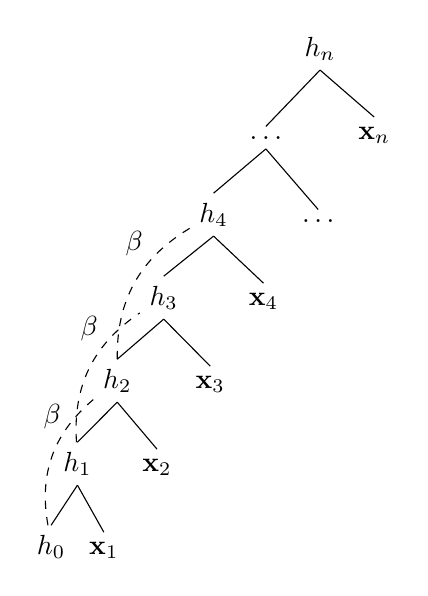
\begin{tikzpicture}
      \Tree [ .$h_n$ [ .$\ldots$ [ .\node(sd){$h_4$}; [ .\node(sc){$h_3$}; [ .\node(sb){$h_2$}; [ .\node(sa){$h_1$}; \node(sz){$h_0$}; $\boldx_1$ ]
      $\boldx_2$ ] $\boldx_3$ ] $\boldx_4$ ] $\ldots$ ] $\boldx_n$ ];
      \draw (sz) edge[dashed, bend left] node[yshift=0.5cm] {$\beta$} (sb);
      \draw (sa) edge[dashed, bend left] node[yshift=0.5cm] {$\beta$} (sc);
      \draw (sb) edge[dashed, bend left] node[yshift=0.5cm] {$\beta$} (sd);
    \end{tikzpicture}
  }
  \end{center}
  \[ \textbf{RNN-DSKIP}(h, \boldx) = \beta \times h + (1-\beta ) \times \tanh( \boldW h + \mathbf{U} \boldx ) \] 
  \[ \beta = NN(h, \boldx) \] 

  \begin{itemize}
  \item Dynamic skip-connections let the network to control \textbf{when} it
    short cuts.
  \end{itemize}
\end{frame}

\begin{frame}{RNN with Gated Skip-Connections}
  \begin{center}
    \scalebox{0.8}{
    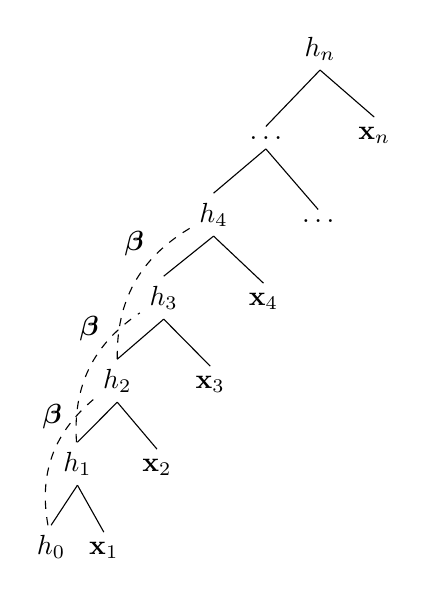
\begin{tikzpicture}
      \Tree [ .$h_n$ [ .$\ldots$ [ .\node(sd){$h_4$}; [ .\node(sc){$h_3$}; [ .\node(sb){$h_2$}; [ .\node(sa){$h_1$}; \node(sz){$h_0$}; $\boldx_1$ ]
      $\boldx_2$ ] $\boldx_3$ ] $\boldx_4$ ] $\ldots$ ] $\boldx_n$ ];
      \draw (sz) edge[dashed, bend left] node[yshift=0.5cm] {$\boldsymbol{\beta}$} (sb);
      \draw (sa) edge[dashed, bend left] node[yshift=0.5cm] {$\boldsymbol{\beta}$} (sc);
      \draw (sb) edge[dashed, bend left] node[yshift=0.5cm] {$\boldsymbol{\beta}$} (sd);
    \end{tikzpicture}
  }
  \end{center}
  \[ \textbf{RNN-GATE}(h, \boldx) = \boldsymbol{\beta}  \odot h + (1-\boldsymbol{\beta} ) \odot \tanh( \boldW h + \mathbf{U} \boldx ) \] 
  \[ \boldsymbol{\beta} = NN(h, \boldx) \] 

  \begin{itemize}
  \item Gates let the network control \textbf{when} and \textbf{what} it shortcuts.
  \end{itemize}
\end{frame}


\begin{frame}{Why gating? }
  \begin{center}
    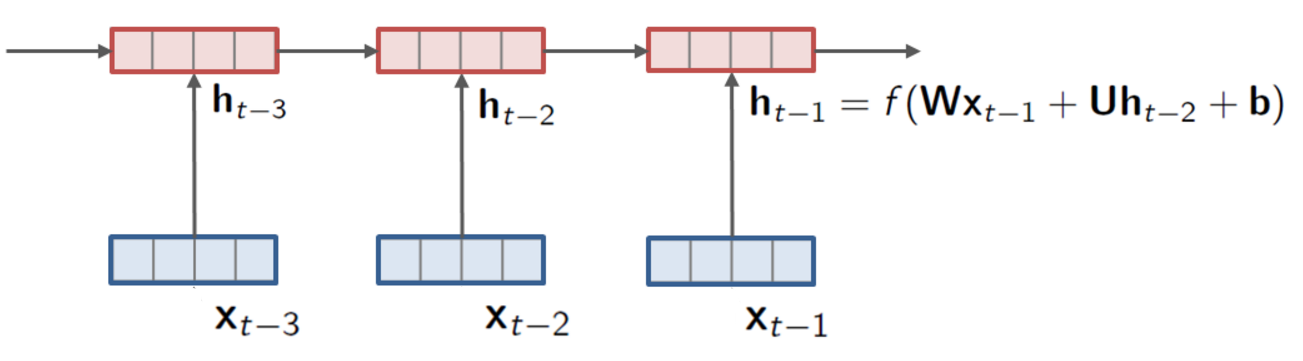
\includegraphics[width=11cm,clip,trim={0 0 15cm 1cm}]{rnn}
  \end{center}  

  \begin{itemize}
  \item Gated RNN can retain the value of important dimensions, and alter others. 
  \item This allows the system to have ``memory'' states.
  \end{itemize}
\end{frame}


\begin{frame}{Sentiment Prediction}
  It has been observed that language models can pick up on 
  sentiment properties. This image shows how one dimension 
  retains sentiment information over time by not updating. 
  
  \begin{center}
    \includegraphics[width=12cm]{sentiment-prediction}
  \end{center}
\end{frame}

\begin{frame}{Long Short-Term Memory}
  The most famous gated RNN is the LSTM. which uses three different 
  types of gates.
\air

  It is complicated to say the least: 

    \begin{eqnarray*}
      \textbf{LSTM}(h_{i-1}, \boldx_i) &=& [\mathbf{c}_i, h_i]  \\
      \mathbf{c}_i &=& \mathbf{j} \odot \mathbf{i}  + \mathbf{ f} \odot \mathbf{ c}_{i-1}    \\
      h_i &=& \tanh(\mathbf{c}_i) \alert{\odot \mathbf{o}}\\ 
      \mathbf{i} &=& \tanh(\boldW^{xi}\boldx  + \boldW^{hi} h_{i-1} + \boldb^i) \\
      \mathbf{j} &=& \sigma(\boldW^{xj} \boldx  + \boldW^{hj} h_{i-1} + \boldb^j) \\
      \mathbf{f} &=& \sigma(\boldW^{xf}\boldx  + \boldW^{hf}h_{i-1} + \boldb^f) \\
      \mathbf{o} &=& \tanh(\boldW^{xo} \boldx  + \boldW^{ho} h_{i-1} + \boldb^o) \\
    \end{eqnarray*}

\end{frame}


\begin{frame}{Schematic View}
  \begin{center}
    \includegraphics[width=13cm]{LSTM3-chain}
  \end{center}
\end{frame}


\begin{frame}{What you should know about LSTMs.}

  \begin{itemize}
  \item  Very effective at language modeling.
    \begin{center}
      \begin{tabular}{lr}
        \toprule
        Language Model & Perplexity \\
        \midrule
        Count-Based &  141 \\    
        LSTM &  78 \\
        \bottomrule
      \end{tabular}
    \end{center}
    \air
    
  \item Seem to better capture long-term dependencies (when necessary) due to gating. 
    \air
  \item If you need to use, details can be abstracted away.
    \begin{center}
      \structure{model.add(LSTM(100))}
    \end{center}
  \end{itemize}
\end{frame}

\begin{frame}
  \centerline{\alert{Example 1}: Synthetic (Finite-State) Language}
  \air

  \begin{center}
    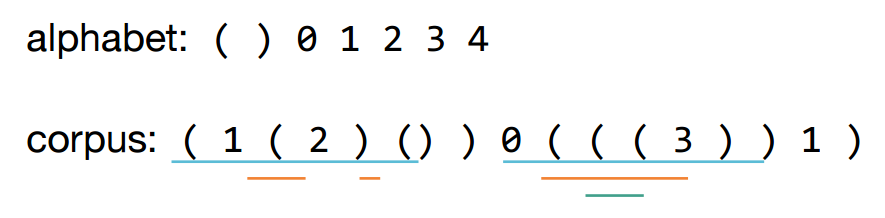
\includegraphics[width=9cm]{parenlang}
  \end{center}
  \mair

  \begin{itemize}
  \item Numbers are randomly generated, must match nesting level.
    \air

  \item Train a predict-next-word language model (decoder-only).
  \end{itemize}
    \[ p(w_t | w_1, \ldots, w_{t-1}) \] 
  
\air
  \centerline{\href[pdfnewwindow=true]{http://lstm.seas.harvard.edu/client/pattern_finder.html?data_set=00parens&source=states::states2&pos=150}{[Parens Example]}}
\end{frame}

\begin{frame}
  \centerline{\alert{Example 2}: Real Language}
  \air

  \begin{description}
  \item[alphabet:] all english words
  \item[corpus:] Project Gutenberg Children's books 
  \end{description}
  % \begin{center}
  %   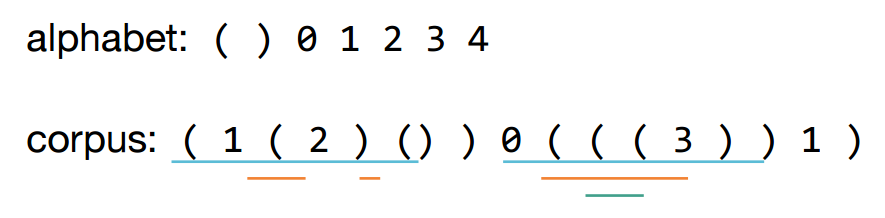
\includegraphics[width=9cm]{parenlang}
  % \end{center}

  \begin{itemize}
  % \item 
  %   \air

  \item Train a predict-next-word language model (decoder-only).

  
  \end{itemize}
    \[ p(w_t | w_1, \ldots, w_{t-1}) \] 

\air
  \centerline{ \href[pdfnewwindow=true]{http://lstm.seas.harvard.edu/client/pattern_finder.html?data_set=05childbook&source=states::states1&pos=100}{[LM Example]}}
\end{frame}

\section{Sequence-to-Sequence}

\begin{frame}{LSTM Language Models}
   We can now estimate, 
  \[ p(w_t | w_1, \ldots, w_{t-1}) \]
  
  So what. This alone is not inherently interesting (even to me).
  \air 
  
  However, what if instead we compute a \textit{conditional} language model.

  \[ p(w_t | w_1, \ldots, w_{t-1}, c) \]

  Where $c$ is the object that we \textit{want to talk about}. 
\end{frame}

\begin{frame}{Machine Translation}
  \begin{itemize}
  \item Supervised machine learning problem, given foreign sentence predict translation.
    \air
  \item Data consists of pairs of French/English data (or any other language 
    pair)
    \air
  \item Classical problem, goes back to the 1950s.
    \air
  \item Modern incarnation is very data driven, tens of millions of sentence pairs.
  \end{itemize}
\end{frame}


\begin{frame}{Back to the Shannon Game}
    \begin{quote}
    THE ROOM WAS NOT VERY LIGHT A SMALL OBLONG READING LAMP ON THE
    DESK SHED GLOW ON POLISHED \_\_\_\
  \end{quote}
  \pause

  But now also assume you know a Spanish version of the sentence:
  \air 

  \begin{quote}
    la habitación no era muy encender una pequeña lámpara de lectura oblonga en el resplandor caseta de escritorio en \textcolor{red}{vidrio} pulido
  \end{quote}

  Call this a \textit{conditional} language modeling problem.

  \[ p(w_t | w_1, \ldots, w_{t-1}, c) \]
\end{frame}


\begin{frame}{Conditional LM}
  Need a neural network to compute the softmax of the next word.
  \[ p(w_t | w_1, \ldots, w_{t-1}, c) \]

  \air
  
  But we now have a general purpose tool for computing a neural network 
  on sequences, the LSTM.
\end{frame}



\begin{frame}{Sequence-to-Sequence }
  \begin{enumerate}
  \item ``Read'' source language sentence with LSTM.
  \item Construct a final source vector representation.
  \item Utilize this vector as part of an LSTM language model.
  \end{enumerate}
  
\end{frame}


\begin{frame}
  \begin{center}
    \structure{Example: Neural Machine Translation \Cite{Sutskever2014}}
  \end{center}
\vspace{-5mm}
 \air
\includegraphics[scale=0.4]{nmt-noattn1}
\end{frame}

\begin{frame}
  \begin{center}
    \structure{Example: Neural Machine Translation \Cite{Sutskever2014}}
  \end{center}
\vspace{-5mm}
 \air
\includegraphics[scale=0.4]{nmt-noattn2}
\end{frame}

\begin{frame}
  \begin{center}
    \structure{Example: Neural Machine Translation \Cite{Sutskever2014}}
  \end{center}
\vspace{-5mm}
 \air
\includegraphics[scale=0.4]{nmt-noattn3}
\end{frame}

\begin{frame}
  \begin{center}
    \structure{Example: Neural Machine Translation \Cite{Sutskever2014}}
  \end{center}
\vspace{-5mm}
 \air
\includegraphics[scale=0.4]{nmt-noattn4}
\end{frame}

\begin{frame}
  \begin{center}
    \structure{Example: Neural Machine Translation \Cite{Sutskever2014}}
  \end{center}
\vspace{-5mm}
 \air
\includegraphics[scale=0.4]{nmt-noattn5}
\end{frame}

\begin{frame}
  \begin{center}
    \structure{Example: Neural Machine Translation \Cite{Sutskever2014}}
  \end{center}
\vspace{-5mm}
 \air
\includegraphics[scale=0.4]{nmt-noattn6}
\end{frame}

\begin{frame}
  \begin{center}
    \structure{Example: Neural Machine Translation \Cite{Sutskever2014}}
  \end{center}
\vspace{-5mm}
 \air
\includegraphics[scale=0.4]{nmt-noattn7}
\end{frame}

\begin{frame}
  \begin{center}
    \structure{Example: Neural Machine Translation \Cite{Sutskever2014}}
  \end{center}
\vspace{-5mm}
 \air
\includegraphics[scale=0.4]{nmt-noattn8}
\end{frame}


\begin{frame}{Sequence-to-Sequence Translation}
  Simple idea, amazing it works at all. 
  \air
  
  \structure{Caveats:}
  
  \begin{itemize}
  \item Needed lots of training data (millions of sentences).
  \item Needed very large models (1000 hidden dimensions, 4 LSTMs stacked). 
  \item Results trailed traditional methods for translation. 
  \end{itemize}
  
  \alert{Argument:}
  \begin{itemize}
  \item Hard to fit entire sentence in a single large vector. 
  \end{itemize}
  
\end{frame}


\section{Sequence-to-Sequence with Attention}


\begin{frame}
  \begin{center}
    \structure{Neural Attention}
    \air


    Input (Foreign sentence) 

    \air 

    \arrowdown  
    \air 

    Memory-Bank Encoder
    \[\text{Encoder}(\text{input}) = h_1, h_2, \dots, h_T  \]

    \air

\pause \arrowdown  

    \air

    \begin{tabular}{cc}
 Attention Distribution  & Context Vector  \\
``where'' & ``what'' \\ 
% $p(z | x, q ; \theta)$  & $c = \sum_{i=1}^T p(z = i | x, q; \theta) x_i$ \\
    \end{tabular}

\air
 
\pause \arrowdown  

    \air

Decoder


% Learn an \textbf{attention} function $\attn(x, q) = [w_1, \dots, w_T]$
% to obtain the weights to be applied to each $h_i$. ($q$ is the 
% \textbf{query vector}. E.g. decoder hidden state in machine translation or the question
% vector in QA)



% \pause \arrowdown  \\ \air
% Obtain the \textbf{context vector} as , use $c$ to predict.
  \end{center}
\end{frame}


\begin{frame}
  \begin{center}
    \structure{Attention-based Neural Machine Translation }
  \end{center}
\center
\vspace{-5mm}
 \air
\includegraphics[scale=0.37]{nmt-attn1}
\end{frame}
\begin{frame}
  \begin{center}
    \structure{Attention-based Neural Machine Translation }
  \end{center}
\center
\vspace{-5mm}
 \air
\includegraphics[scale=0.37]{nmt-attn2}
\end{frame}
\begin{frame}
  \begin{center}
    \structure{Attention-based Neural Machine Translation }
  \end{center}
\center
\vspace{-5mm}
 \air
\includegraphics[scale=0.37]{nmt-attn3}
\end{frame}
\begin{frame}
  \begin{center}
    \structure{Attention-based Neural Machine Translation }
  \end{center}
\center
\vspace{-5mm}
 \air
\includegraphics[scale=0.37]{nmt-attn4}
\end{frame}
\begin{frame}
  \begin{center}
    \structure{Attention-based Neural Machine Translation }
  \end{center}
\center
\vspace{-5mm}
 \air
\includegraphics[scale=0.37]{nmt-attn5}
\end{frame}
\begin{frame}
  \begin{center}
    \structure{Attention-based Neural Machine Translation }
  \end{center}
\center
\vspace{-5mm}
 \air
\includegraphics[scale=0.37]{nmt-attn6}
\end{frame}
\begin{frame}
  \begin{center}
    \structure{Attention-based Neural Machine Translation }
  \end{center}
\center
\vspace{-5mm}
 \air
\includegraphics[scale=0.37]{nmt-attn7}
\end{frame}
\begin{frame}
  \begin{center}
    \structure{Attention-based Neural Machine Translation }
  \end{center}
\center
\vspace{-5mm}
 \air
\includegraphics[scale=0.37]{nmt-attn8}
\end{frame}
\begin{frame}
  \begin{center}
    \structure{Attention-based Neural Machine Translation }
  \end{center}
\center
\vspace{-5mm}
 \air
\includegraphics[scale=0.37]{nmt-attn9}
\end{frame}
\begin{frame}
  \begin{center}
    \structure{Attention-based Neural Machine Translation }
  \end{center}
\center
\vspace{-5mm}
 \air
\includegraphics[scale=0.37]{nmt-attn10}
\end{frame}


\begin{frame}
  \begin{center}
    \structure{Attention Networks: Notation}

    \air 
    \air 

  \begin{tabular}{cl}
    $x_1, \ldots, x_T $ & Memory bank (``what'') \\
    $q$ &Query \\
    $z$ &Memory selection (random variable)  \\ 
    $p(z \given x, q; \theta)$ & Attention distribution (``where'') \\ 
    $c  =\mathbb{E}_{z \given x, q } [x_z]  $ & Context Vector \\
  \end{tabular}
  \end{center}
\air 

% \pause
% End-to-End Requirements:
%   \begin{enumerate}
%   \item Need to compute attention $p(z=i \given x, q; \theta)$
%   \item Need to backpropagate to learn parameters $\theta$ 
%   \end{enumerate}

% The \textbf{context} vector $c$ is
% defined as the ``expected annotation'',
% \[c  =\E_{z \sim p(z \given x, q )} [f(x,z)]  \] 

\end{frame}

\begin{frame}
  \begin{center}
    \structure{Attention Networks: Machine Translation}
  \end{center}

  \begin{center}
    \begin{tabular}{cll}
      $x_1, \ldots, x_T$ & Memory bank& Source RNN hidden states \\
      $q$& Query &Decoder hidden state \\
      $z$& Memory selection & Source position $\{1, \dots, T\}$ \\
      $p(z=i \given x, q; \theta)$ & Attention distribution & $\softmax (x_i^\top q)$  \\ 
    $c  =\mathbb{E} [x_z]  $ & Context Vector & \\
    \end{tabular}    
  \end{center}

\end{frame}



\begin{frame}{Google NMT}
  \begin{center}
    \includegraphics[width=12cm]{gnmt}
  \end{center}
\end{frame}

\section{Applications}

\begin{frame}{}
  \begin{center}
    \structure{Encoder-Decoder with Attention}
  \end{center}


  \begin{itemize}
  \item \structure{Machine Translation}
    \vspace{0.5cm}

  \item Question Answering 
  \item Natural Language Inference 
  \item Algorithm Learning
  \item Parsing 
  \item Speech Recognition 
  \item Summarization 
  \item Caption Generation
  \item and more... 
  \end{itemize}
  
\end{frame}

\begin{frame}
  \begin{center}
    \structure{Other Applications: Image Captioning }
  \end{center}
\center
\includegraphics[width=11cm]{attn-example2}
\end{frame}


\begin{frame}
  \begin{center}
    \structure{Other Applications: Speech Recognition }
  \end{center}
\center
\includegraphics[width=11cm]{attn-example3}
\end{frame}

\begin{frame}
  \begin{center}
    \structure{Applications From HarvardNLP: Summarization }
  \end{center}
\center
\includegraphics[width=8cm]{attn-example5}
\end{frame}

\begin{frame}
  \begin{center}
    \structure{Applications From HarvardNLP: Image-to-Latex }
  \end{center}
\center
\includegraphics[width=11cm]{attn-example4}
\end{frame}

\begin{frame}
  \begin{center}
    \includegraphics[width=6cm]{network}
  \end{center}
\end{frame}

\begin{frame}
  \begin{center}
    \structure{Applications From HarvardNLP: OpenNMT}
  \end{center}
\center
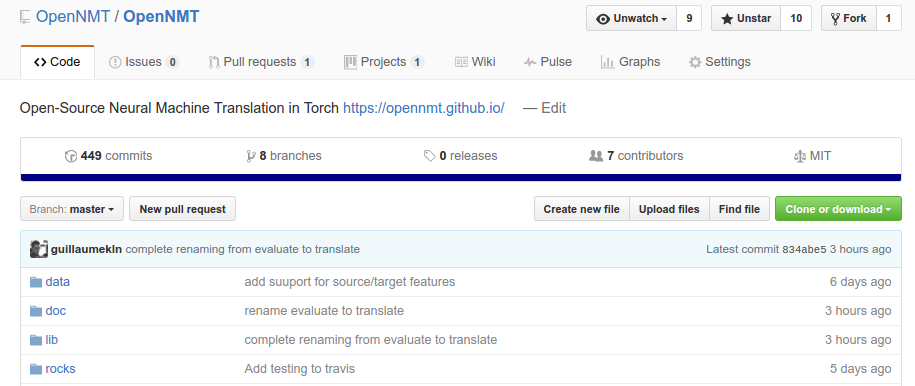
\includegraphics[width=11cm]{opennmt}
\end{frame}



% \begin{frame}
%   \[ \textbf{Avg}(h, \boldx) = \tanh(\boldW h + \mathbf{U} \boldx + \boldb) \] 

%   \[ \textbf{RNN}(h, \boldx) = \tanh(\boldW h + \mathbf{U} \boldx + \boldb) \] 
% \end{frame}

% \begin{frame}
%   \begin{center}
%     
\includegraphics[width=12cm]{nytai}

%     (December, 2016)
%   \end{center}
% \end{frame}

% \begin{frame}
%   \begin{center}
%     \structure{Machine Translation}
%   \end{center}
%   \begin{center}
%     \includegraphics[width=12cm]{nmtexamples}
%   \end{center}
% \end{frame}


% \begin{frame}
%   \begin{center}
%     \structure{Machine Translation}
%   \end{center}
%   \begin{center}
%     \includegraphics[width=12cm]{nmtexamples2}
%   \end{center}
% \end{frame}

% \begin{frame}
%   \begin{center}
%     \structure{Other Applications: Image Captioning \Cite{Xu2015}}
%   \end{center}
% \center
% \includegraphics[width=11cm]{attn-example2}
% \end{frame}


% \begin{frame}
%   \begin{center}
%     \structure{Other Applications: Speech Recognition \Cite{Chan2015}}
%   \end{center}
% \center
% \includegraphics[width=11cm]{attn-example3}
% \end{frame}


% \begin{frame}
%   \begin{center}
%     \textbf{Language Models}
%   \end{center}
% \end{frame}

% \begin{frame}
%   \only<1>{
%   \begin{center}
%     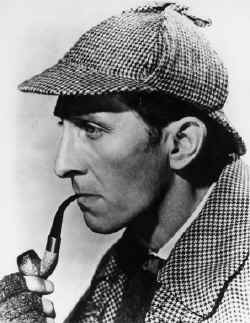
\includegraphics[width=3cm]{holmes}
%   \end{center}
% }
% \only<2>{
%   \begin{center}
%     \begin{tikzpicture}[spy using outlines={circle, magnification=20,
%         size=3cm, connect spies}]
%       \node {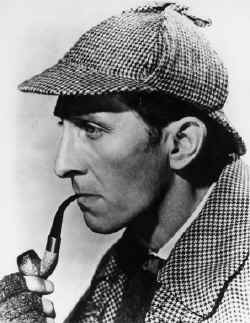
\includegraphics[width=3cm]{holmes}}; 
%       \spy [cyan] on
%       (0.0,0.3) in node [left] at (5.4,-1.15);
%     \end{tikzpicture}
%   \end{center}
% }
%   \begin{quote}
%     It is a capital mistake to theorize before one has
%     data. Insensibly one begins to twist facts to suit theories,
%     instead of theories to suit facts. -Sherlock Holmes, A Scandal in Bohemia
%   \end{quote}


% \end{frame}

% \begin{frame}

%   % \begin{center}
%   %   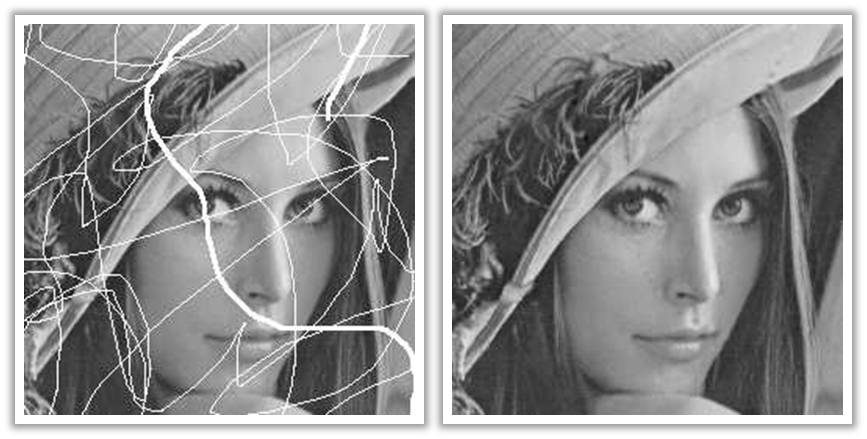
\includegraphics[width=6cm]{lena}
%   % \end{center}

%   \air
%   \only<1> {
%     \begin{quote}
%     It is a capital mistake to theorize before one has \_\_\_\_\_\_ $\ldots$ 
%     \end{quote}
%   }
%   \only<2> {
%     \begin{quote}
%       108 938 285 28 184 29 593 219 58 772 \_\_\_\_\_\_ $\ldots$ 
%     \end{quote}    
%   }
% \end{frame}



% \begin{frame}
%   \begin{center}
%     \structure{Language Modeling Task}
%   \end{center}
%   Given a sequence of text give a probability distribution 
%   over the next word. 

% \air

%   The Shannon game. Estimate the probability of the next letter/word
%   given the previous.

%   \begin{quote}
%     THE ROOM WAS NOT VERY LIGHT A SMALL OBLONG READING LAMP ON THE
%     DESK SHED GLOW ON POLISHED \_\_\_\
%   \end{quote}


% \end{frame}


% \begin{frame}
%   \begin{center}
%     \structure{Shannon (1948) \textit{Mathematical Model of Communication}}
%   \end{center}
% \air
  
% \begin{quote}  
%   We may consider a discrete source, therefore,
% to be represented by a stochastic process. Conversely, any stochastic
% process which produces a discrete sequence of symbols chosen from a finite
% set may be considered a discrete source. This will include such cases as:

% 1. Natural written languages such as English, German, Chinese.
% ...
% \end{quote}
% \end{frame}

% \begin{frame}[allowframebreaks]
%   \begin{center}
%     \structure{Shannon's Babblers}
%   \end{center}
%   \begin{quote}
   
%   4. Third-order approximation (trigram structure as in English).

% IN NO 1ST LAT WHEY CRATICT FROURE BIRS GROCID
% PONDENOME OF DEMONSTURES OF THE REPTAGIN IS
% REGOACTIONA OF CRE
%   \end{quote}

%   \begin{quote}
% 5. First-Order Word Approximation. Rather than continue with tetragram,
% ... , II-gram structure it is easier and better to jump at this
% point to word units. Here words are chosen independently but with
% their appropriate frequencies.

% REPRESENTING AND SPEEDILY IS AN GOOD APT OR
% COME CAN DIFFERENT NATURAL HERE HE THE A IN
% CAME THE TO OF TO EXPERT GRAY COME TO FURNISHES
% THE LINE MESSAGE HAD BE THESE.

%   \end{quote}

%   \begin{quote}
%     6. Second-Order Word Approximation. The word transition probabilities
% are correct but no further structure is included.

% THE HEAD AND IN FRONTAL ATTACK ON AN ENGLISH
% 'RITER THAT THE CHARACTER OF THIS POINT IS
% THEREFORE ANOTHER METHOD FOR THE LETTERS
% THAT THE TIME OF WHO EVER TOLD THE PROBLEM
% FOR AN UNEXPECTED

% The resemblance to ordinary English text increases quite noticeably at
% each of the above steps.

%   \end{quote}
% \end{frame}

% % \begin{frame}
% %   \begin{center}
% %     \textbf{Simple Language Models}
% %   \end{center}
% % \end{frame}


% \begin{frame}

% Goal: Estimate Markov model 
% \[ p(w_{t} | w_{1}, \ldots, w_{t-1}) \approx p(w_{t} | w_{t-n}, \ldots w_{t-1})\] 

% Ingredients: 

% \begin{itemize}
% \item 1 Corpus (e.g. the entire web)

% \end{itemize}

% Steps:

% \begin{itemize}
% \item (1) Collect words, (2) Count up n-grams, (3) Divide$^*$
%   \begin{eqnarray*} 
%     p(w_{t+1} | w_{t-n+1}, \ldots w_{t}) &=& \frac{\#( w_{t-n+1}, \ldots, w_{t+1}) }{\#( w_{t-n+1}, \ldots, w_{t})} \\
%     &=&  \frac{\#(\mathrm{theorize\ before\ one\ has\ data})}{\#(\mathrm{theorize\ before\ one\ has})}
%     \end{eqnarray*}
% \end{itemize}
% \end{frame}

% \begin{frame}
%   \begin{center}
%     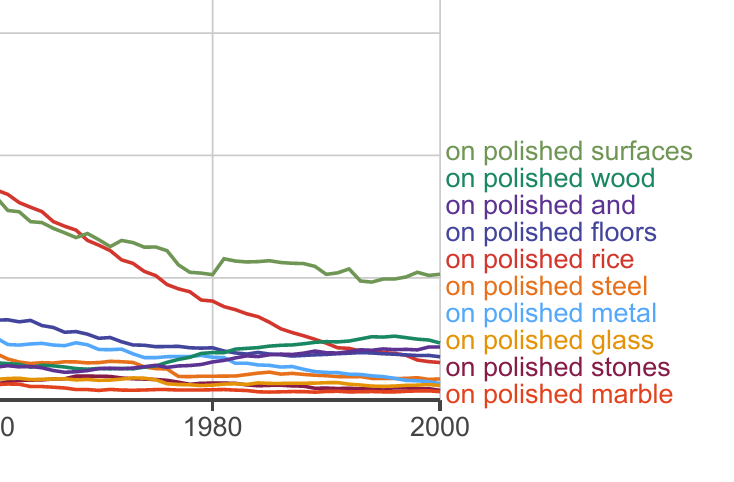
\includegraphics[width=\textwidth]{polished}
%   \end{center}
% \end{frame}


% \begin{frame}
%   \begin{center}
%     \alert{Google 1T}

%   \end{center}
%   \begin{table}
%     \centering
%   \begin{tabular}{ll}
%     \toprule
%     Number of token  &1,024,908,267,229 \\
%     Number of sentences & 95,119,665,584 \\
%     Size compressed (counts only) & 24 GB \\  
%     \midrule
%     Number of unigrams & 13,588,391 \\
%     Number of bigrams & 314,843,401 \\ 
%     Number of trigrams & 977,069,902 \\ 
%     Number of fourgrams & 1,313,818,354 \\
%     Number of fivegrams&  1,176,470,663 \\
%     \bottomrule
%   \end{tabular}
%   \end{table}


% \end{frame}

% \begin{frame}
%   \textbf{Zipf' Law (1935,1949):}
%   \begin{quote}
%     The frequency of any word is inversely proportional to its rank in the frequency table.
%   \end{quote}


%      \begin{center}
%        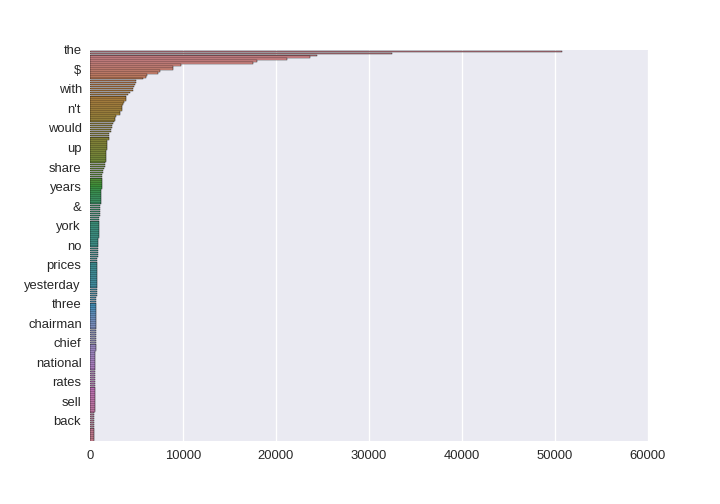
\includegraphics[width=0.8\textwidth]{zipf}         
%      \end{center}
% \end{frame}


% \begin{frame}
%   \begin{center}
%     \textbf{Neural Networks}
%   \end{center}
% \end{frame}

% \begin{frame}{Intuition: N-Gram Issues}
  
%   Training: 

%   \begin{center}
%     the arizona corporations commission \alert{authorized}
%   \end{center}

%   Test: 
%   \begin{center}
%     the colorado businesses organization \alert{\_\_\_}
%   \end{center}
%   \pause 
  
%   \begin{itemize}
%   \item Does this training example help here?
%     \begin{itemize}
%     \item Not really. No count overlap.
%     \end{itemize}
%     \air 
%     \pause 
%   \item Intuition: hope to learn that similar words act similarly. 
%   \end{itemize}
% \end{frame}


% \begin{frame}{Alternative Approach}

%   Treat as multi-class prediction!

%   \air

%   Let $\mcV$ be all possible words in the language (English 10,000 - 100,000). 
%   Predict over words.

% \air

%  Important ideas that you have seen .

%   \begin{enumerate}


%   \item \textbf{Neural Network} to learn feature representation. 
%   \item \textbf{Softmax} for multiclass prediction of next word (out of $\mcV$ )
%   \item \textbf{Cross-entropy} loss as training objective.
%   \end{enumerate}
% \end{frame}


% \begin{frame}{Language Modeling as Supervised Learning}
%   \begin{quote}
%     THE ROOM WAS NOT VERY LIGHT A SMALL OBLONG READING LAMP ON THE
%     DESK SHED GLOW ON POLISHED \_\_\_\
%   \end{quote}


%   \begin{itemize}
%   \item Training data is pairs are $(w_t, \{w_{t-3}, w_{t-2}, w_{t-1}\})$.

%   \item Input is sentence up until the blank, output is next word
%     prediction.
%   \item Challenging multi-class prediction problem, feature representation matters.

%     \pause
%     Neural Network 

%     \[ p(w_t | \{w_{t-3}, w_{t-2}, w_{t-1}\} ) = \sigma(z)_{w_t} \]
%     where 
%     \[z = NN(\{w_{t-3}, w_{t-2}, w_{t-1}\}) \]
%   \end{itemize}
% \end{frame}

% \begin{frame}
%   A \structure{neural network} is a \alert{function approximator}

  
%   \begin{itemize}
%   \item  $NN(\boldx; \theta)$; a learned function from $\boldx$ with parameters $\theta$.
%   \end{itemize}
% % \end{frame}

% % \begin{frame}{Neural Network}

%   \[NN_{MLP1}(\boldx) =  \boldW^2 \tanh(\boldW^1 \boldx + \boldb^1) + \boldb^2\]
%   \begin{itemize}
%   \item $\boldx$; input

%   \item $\boldW, \boldb$; parameters
%   % \item $\boldW^1 \in \reals^{\din \times \dhid}, \boldb^1 \in \reals^{1 \times \dhid}$; first affine transformation
%   % \item $\boldW^2 \in \reals^{\dhid \times \dout}, \boldb^2 \in \reals^{1 \times \dout}$; second affine transformation
%   \item $\tanh$ is \textit{non-linearity} 
%   % \item $g(\boldx\boldW^1 + \boldb^1)$ is the \textit{hidden layer}
%   \end{itemize}
%   \begin{figure}
%     \centering
%     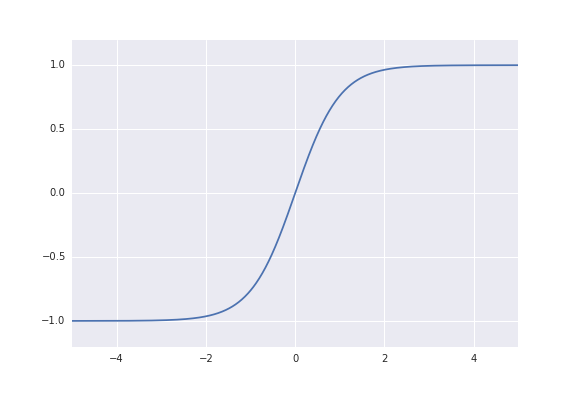
\includegraphics[width=5cm]{tanh}     
%   \end{figure}

% \end{frame}


% \begin{frame}
%     \begin{figure}
%     \centering
%     \includegraphics[width=8cm]{08-nn}
%     \end{figure}
% \end{frame}


% \begin{frame}{Word Representation}
%   \begin{itemize}
%   \item How can a word be fed into a neural network?

%   \item Each word has an associated numerical index, not like images or 
%     sounds.

%   \item Need a way to know if two words are ``close'' to each other 
%     for the network. 
%   \end{itemize}

% \end{frame}


% \begin{frame}{Words Embeddings}
%   \begin{center}
%     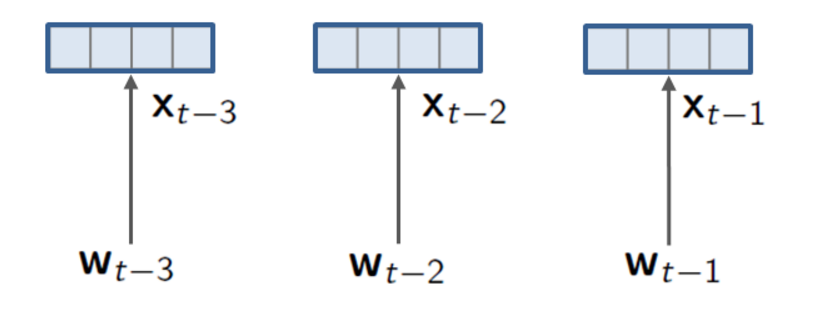
\includegraphics[width=7cm]{emb}
%   \end{center}
%   \begin{itemize}
%   \item Associate each words with an \textit{embedding} vector, e.g. in 50 dimensions. 
%   \item Store this in a big table. 
%   \item ``Move'' the vectors around based on backpropagation, i.e. if the model 
%     makes the wrong prediction the vector associated with a word is updated.
%   \end{itemize}
% \end{frame}



% % \begin{frame}{Word Embeddings}
  
% % \end{frame}

% % \begin{frame}
% %   \begin{center}
% %     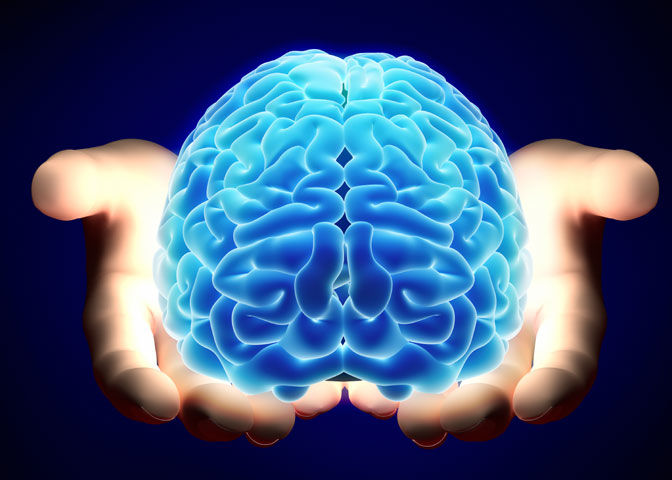
\includegraphics[width=5cm]{brain}
% %   \end{center}
% % \end{frame}








% % \begin{frame}
% %   Logistic sigmoid function:
% %   \[\sigma(t) = \frac{1}{1 + \exp(-t)} \]
% %   \begin{figure}
% %     \centering
% %     \includegraphics[width=5cm]{sigmoid}     
% %   \end{figure}

% %   \begin{itemize}
% %   \item $\sigma((\boldW^1 \boldx + \boldb^1)_i)$
% %   \end{itemize}
% % \end{frame}




% % \begin{frame}{Softmax}
  
% % \end{frame}



% % \begin{frame}
% %   \begin{center}


% %   \begin{tikzpicture}
% %     \node(aa)[draw, circle]{$x_1$};
% %     \node(ab)[below of =  aa, draw, circle]{$x_2$};
% %     \node(ac)[below of = ab, draw,circle]{$x_3$};
% %     \node(ad)[below of = ac]{$\vdots$};
% %     \node(ae)[below of =  ad, draw, circle]{$x_{\din}$};


% %     \node(ba)[xshift= 2cm, yshift=-0.5cm, right of = aa, draw, circle]{$h_1$};
% %     \node(bb)[below of =  ba, draw, circle]{$h_2$};
% %     \node(bc)[below of = bb]{$\vdots$};

% %     \node(bd)[below of =  bc, draw, circle]{$h_{\dhid}$};

% %     \path[draw] (aa) -- (ba);
% %     \path[draw] (aa) -- (bb);
% %     \path[draw] (aa) -- (bd);

% %     \path[draw] (ab) -- (ba);
% %     \path[draw] (ab) -- (bb);
% %     \path[draw] (ab) -- (bd);

% %     \path[draw] (ac) -- (ba);
% %     \path[draw] (ac) -- (bb);
% %     \path[draw] (ac) -- (bd);

% %     \path[draw] (ae) -- (ba);
% %     \path[draw] (ae) -- (bb);
% %     \path[draw] (ae) -- (bd);


% %     \node(ca)[xshift= 2cm, yshift=0.5cm, right of = ba, draw, circle]{$z_1$};
% %     \node(cb)[below of =  ca, draw, circle]{$z_2$};
% %     \node(cc)[below of =  cb, draw, circle]{$z_3$};
% %     \node(cd)[below of = cc]{$\vdots$};
% %     \node(ce)[below of =  cd, draw, circle]{$z_{\dout}$};


% %     \path[draw] (ba) -- (ca);
% %     \path[draw] (ba) -- (cb);
% %     \path[draw] (ba) -- (cc);
% %     \path[draw] (ba) -- (ce);

% %     \path[draw] (bb) -- (ca);
% %     \path[draw] (bb) -- (cb);
% %     \path[draw] (bb) -- (cc);
% %     \path[draw] (bb) -- (ce);

% %     \path[draw] (bd) -- (ca);
% %     \path[draw] (bd) -- (cb);
% %     \path[draw] (bd) -- (cc);
% %     \path[draw] (bd) -- (ce);


% %   \end{tikzpicture}
% %   \end{center}j
% % \end{frame}


% % \begin{frame}{Interpretation of Network}

% %   \begin{itemize}
% %   \item Notation input $\reals^m$ and basis $\reals^d$.  
% %   \item Unlike other problems here $m$ is large $|\mcV|$ (10,000-100,000)
% %   \item But $d$ can be much smaller. Why is that?  
  
% %   \air
% %   \[\boldW^1 \begin{bmatrix}0 \\ 0\\ 1 \\ \vdots \\0 \\\end{bmatrix} = \boldW^1_{\star, j} \] 
      
% %   \item The output of this layer $\boldW^1_{\star, j} \in \reals^d$ is called a \textit{word vector}. 
% %   \end{itemize}
% % \end{frame}

% % \begin{frame}{Sparse versus Distributed Representation}
% %   \begin{itemize}
% %   \item Internally we have now seen two representations of words 

% %   \item $\boldx$ Sparse:  Very high dimensional, easy to get back the original word, 
% %     but feature weights are not shared between words. $\boldw_j$ is weight for 
% %     one word. 
% %     \[ [0, 0, 0, 1, \ldots 0] \] 
% %     \pause 

% %   \item $\bphi(\boldx)$ Distributed:  Low dimensional but dense, each dimension is a feature of the 
% %     word, $\boldw_j$ is weight for basis function. 
% %     \[ [0.23, 0.32, 0.109, -0.1231, \ldots, 0.402] \] 

% %   \end{itemize}
% % \end{frame}




% % \begin{frame}
% %   \begin{center}
% %     \textbf{Neural Networks for Language}
% %   \end{center}
  
% %   \begin{itemize}
% %   \item $\boldx$; previous words 
% %   \item $NN(\boldx)$; score for next word  
% %   \end{itemize}
% %   \[NN_{MLP1}(\boldx) =  \boldW^2 \sigma(\boldW^1 \boldx + \boldb^1) + \boldb^2\]

% %   \begin{center}
% %     \begin{tikzpicture}
% %     \node(aa)[draw, circle]{$x_1$};
% %     \node(ab)[below of =  aa, draw, circle]{$x_2$};
% %     \node(ac)[below of = ab, draw,circle]{$x_3$};
% %     \node(ad)[below of = ac]{$\vdots$};
% %     \node(ae)[below of =  ad, draw, circle]{$x_{n}$};


% %     \node(ba)[xshift= 2cm, yshift=-0.5cm, right of = aa, draw, circle]{$h_1$};
% %     \node(bb)[below of =  ba, draw, circle]{$h_2$};
% %     \node(bc)[below of = bb]{$\vdots$};

% %     \node(bd)[below of =  bc, draw, circle]{$h_{d}$};

% %     \path[draw] (aa) -- (ba);
% %     \path[draw] (aa) -- (bb);
% %     \path[draw] (aa) -- (bd);

% %     \path[draw] (ab) -- (ba);
% %     \path[draw] (ab) -- (bb);
% %     \path[draw] (ab) -- (bd);

% %     \path[draw] (ac) -- (ba);
% %     \path[draw] (ac) -- (bb);
% %     \path[draw] (ac) -- (bd);

% %     \path[draw] (ae) -- (ba);
% %     \path[draw] (ae) -- (bb);
% %     \path[draw] (ae) -- (bd);


% %     \node(ca)[xshift= 2cm, yshift=0.5cm, right of = ba, draw]{word 1};
% %     \node(cb)[below of =  ca, draw]{word 2};
% %     \node(cc)[below of =  cb, draw]{word 3};
% %     \node(cd)[below of = cc]{$\vdots$};
% %     \node(ce)[below of =  cd, draw]{word n};


% %     \path[draw] (ba) -- (ca);
% %     \path[draw] (ba) -- (cb);
% %     \path[draw] (ba) -- (cc);
% %     \path[draw] (ba) -- (ce);

% %     \path[draw] (bb) -- (ca);
% %     \path[draw] (bb) -- (cb);
% %     \path[draw] (bb) -- (cc);
% %     \path[draw] (bb) -- (ce);

% %     \path[draw] (bd) -- (ca);
% %     \path[draw] (bd) -- (cb);
% %     \path[draw] (bd) -- (cc);
% %     \path[draw] (bd) -- (ce);
% %   \end{tikzpicture}
% % \end{center}
% % \end{frame}



% \begin{frame}
%   \begin{center}
%     \includegraphics[height=0.9\textheight]{graph}

%     \href[pdfnewwindow=true]{http://harvardnlp.github.io/seq2seq-talk/web/wordvecs.html}{[Words Vectors]}
%    \end{center}
% \end{frame}


% \begin{frame}{Notable Properties}
%   After applying PCA to word embeddings
%   \air 
%   \begin{center}
%     \includegraphics[width=7cm]{athletes}
%   \end{center}
% \end{frame}




% \begin{frame}{Modern Word Vectors}  
%   [Demo: TensorBoard]
% \end{frame}


% \begin{frame}{Language Modeling with Neural Networks}
%   Recall the definition of the \textbf{softmax}, with $z$ the representation 
%   of the context.

%   \air


%   \begin{center}
%     \includegraphics[width=5cm]{softmax}
%   \end{center}
% \air

%   \[ \sigma(z)_j = \frac{e^{z_j}}{\sum_{k=1}^Ke^{z_{k}}}  \] 
%   For language modeling $K$ is huge! Need to compute for the full
%   vocabulary.
%   \air

%   Became possible to do with refinement of GPUs.
% \end{frame}


% \begin{frame}{Problems With MLP Language Models}  
%   MLP language models provide a way to learn 
%   representations of words.

%   \begin{itemize}
%   \item Can be trained as a standard neural network.
%   \item Allows us to learn words are similar. 
%   \end{itemize}

%   \air

%   Still have several \alert{issues}.

%   \begin{itemize}
%   \item Have to differentiate between locations (2 words back, 5 words back).
%   \item Only have a fixed amount of history. 
%   \end{itemize}
% \end{frame}

% \begin{frame}
%   \begin{center}
%     \textbf{Recurrent Neural Networks Models}
%   \end{center}
% \end{frame}

% \begin{frame}{Recurrent Neural Networks}
%   \textbf{Main Idea:} Build neural networks that are deep \textit{in time.}

%   \begin{itemize}
%   \item   Deep MLP/CNN: Stack multiple non-linear network units on-top of 
%     input. Learn richer feature representations. 

%   \item RNN: Use a non-linear transformations based on each input in a time-series.
    
%   \end{itemize}

% \end{frame}
% \begin{frame}{RNN versus Deep Convolution}
%   \begin{columns}
%     \column{0.5\textwidth}

%     \begin{center}
%       \textbf{Convolution}
%       \air

%       \Tree [ .$NN_{Conv}$ [ .$Pool$ [ .$NN_{Conv}$ $\boldx_1$ $\boldx_2$ $\ldots$
%       $\boldx_n$ ] ] ] 
%     \end{center}
%     \column{0.5\textwidth}

%     \begin{center}
%       \textbf{RNN}
%       \air 

%       \Tree [ .$h_n$ [ .$\ldots$ [ .$h_3$ [ .$h_2$ [ .$h_1$ $h_0$ $\boldx_1$ ]
%       $\boldx_2$ ] $\boldx_3$ ] $\ldots$ ] $\boldx_n$ ]
%     \end{center}
%   \end{columns}
% \end{frame}


% \begin{frame}{RNN Mathematically}


%   Let $h_0 \gets 0$, 
%   \[ h_1 \gets \textbf{RNN}(h_{0}, \boldx_1;\theta) \] 
%   \[ h_2 \gets \textbf{RNN}(h_{1}, \boldx_2;\theta) \] 
%   \[ h_3 \gets \textbf{RNN}(h_{2}, \boldx_3;\theta) \] 
%   \centerline{$\vdots$}
%   \[ h_n \gets \textbf{RNN}(h_{n-1}, \boldx_n;\theta) \] 
  
%   Where RNN is a neural network layer with the same weights $\theta$ applied 
%   at each time step, for instance: 
  
%   \[ \textbf{RNN}(h, \boldx) = \tanh(\boldW^a h + \boldW^{b} x ) \] 

% \end{frame}


% % \begin{frame}
  
% % \end{frame}

% \begin{frame}{Why RNN?}
  
%   \begin{itemize}
%   \item Get a single hidden vector for each time step. 
%   \item Vector can learn to capture important properties of the previous inputs.  
%   \item May allow us to make prediction based on history.
%   \end{itemize}
% \end{frame}

% % \begin{frame}
% %     \begin{center}
% %     \textbf{This Talk: Neural Networks For Language}
% %   \end{center}
% % \end{frame}

% \begin{frame}%{Deep Learning Toolbox}
%   \begin{center}
%     \alert{RNN For Language Modeling}
%     \air 
%   \end{center}
%   \begin{center}
%     \begin{tabular}{cclll}
%       \structure{Embeddings} & & words &$\Rightarrow$& word vectors \\\\
%       % \structure{Convolutions} &&  feature n-grams & $\Rightarrow$& dense features  \\\\

%       \structure{RNNs} & & word vectors & $\Rightarrow$ & hidden states  \\\\
%       \structure{Softmax} & & hidden states & $\Rightarrow$ & word prediction \\
%     \end{tabular}
%   \end{center}

% \end{frame}


% \begin{frame}{Words Embeddings}
%   \begin{center}
%     \includegraphics[width=7cm]{emb}
%   \end{center}
%   \begin{itemize}
%   \item Map words to vector space, just as before. 
%   \end{itemize}

% \end{frame}

% \begin{frame}{RNN}
%   \begin{center}
%     \includegraphics[width=11cm]{rnn}
%   \end{center}  
%   \begin{itemize}
%   \item Apply recurrent neural network over vector space of words to create hidden states.
%   \end{itemize}
% \end{frame}




% \begin{frame}{Softmax}
%   \begin{center}

%     \includegraphics[width=0.8\textwidth]{rnnlm5}
%   \end{center}
    
%   \begin{itemize}
%   \item Compute softmax over all possible next words to predict.
%   \end{itemize}
%   \[  p(w_t \given w_1, \ldots, w_{t-1}) = \sigma(\mathbf{W} \mathbf{h}_{t-1} + \mathbf{b})_w \] 

%   % \[ p(w_{1:T} ) = \prod_{t} p(w_t | w_1, \ldots, w_{t-1}) \] 
%     % \caption{Xu et al (2015)}  
% \end{frame}


% \begin{frame}
%   % \begin{frame}
%   \begin{center}
%     \includegraphics[width=\textwidth]{lstm1}


%     {\footnotesize (Karpathy et al, 2015)}
%   \end{center}
%     % \caption{Xu et al (2015)}  
% \end{frame}

% \begin{frame}{How do we learn the model?}
%   \begin{itemize}
%   \item RNNs are trained with SGD and Backprop (surprise)
%     \air 

%   \item Implementation can be complicated, mainly for efficiency.
%     \air

%   \item Called \textit{backpropagation through time} (BPTT).
%   \end{itemize}
% \end{frame}

% % \begin{frame}{Training Acceptors}
% %   Training process:
% %   \begin{itemize}
% %   \item Run forward propagation.
% %     \air 
% %   \item Run backward propagation.
% %     \air

% %   \item Update all weights
% %   \end{itemize}

% %   Weights $\theta$ of $R$ are shared:
% % \end{frame}

% \begin{frame}{BPTT (One Word)}
%   \begin{itemize}
%   \item \alert{Run forward propagation}.
%   \item \structure{Run backward propagation}.
%   \item Update all weights (shared)
%   \end{itemize}

%     \begin{center}
%       \scalebox{0.7}{\Tree [  .\alert<5->{\structure<6->{$\hat{\boldy}$}} [ .$\alert<4->{\structure<7->{h_n}}$ [ .$\ldots$ [ .$\alert<3->{\structure<8->{h_3}}$ [ .$\alert<2->{\structure<9->{h_2}}$ [ .$\alert<1->{\structure<10->{h_1}}$ $h_0$ $\boldx_1$ ]
%       $\boldx_2$ ] $\boldx_3$ ] $\ldots$ ] $\boldx_n$ ] ]}
%     \end{center}
% \end{frame}


% \begin{frame}{Issues}
%   \begin{itemize}
%   \item Can be inefficient, but batch/GPUs help.
%     \air

%   \item Model is much deeper than previous approaches.
%     \begin{itemize}
%     \item This matters a lot, focus of next class.
%     \end{itemize}
%     \air

%   \item Variable-size model for each sentence.
%     \begin{itemize}
%     \item Have to be a bit more clever in Keras.
%     \end{itemize}
%   \end{itemize}
% \end{frame}

% \begin{frame}{Application of RNNs}
%   RNN models have lead to a \textbf{major} increase in the accuracy of 
%   language models.

%   \begin{center}
%     Why did this matter?
%   \end{center}
%   \pause

%   \begin{center}
%     \includegraphics<2>[width=9cm]{drumpf}
%   \end{center}
% \end{frame}



% \begin{frame}{Language Modeling Applications}

%   \begin{columns}    
%     \begin{column}{0.5\textwidth}
%   \begin{itemize}
%   \item Speech Recognition
%   \item Machine Translation
%   \item Summarization
%   \item Dialogue
%   \item Soft Keyboards
%   \item Word Correction
%   \item Text Simplification
%   \item $\ldots$
%   \end{itemize}
%   \end{column}


%     \begin{column}{0.5\textwidth}
%       \vspace{2cm}
     
%       \includegraphics[width=5cm]{siri}
%     \end{column}
%   \end{columns}

% \end{frame}

% \begin{frame}{Next Class}
  
%   \begin{itemize}
%   \item Easier to train variants of RNN (Long-Short Term Memory)
%   \item LSTMs for Machine Translation 
%   \item Many Cool Applications...
%   \end{itemize}

% \end{frame}





% \begin{frame}
% \begin{center}
% Thanks!
% \end{center}
% \end{frame}


% % \begin{frame}
% %   \begin{center} 
% %     \structure{Thank You}
% %   \end{center}
% %   \air 
% %   \begin{center}
% %     \includegraphics[width=3cm]{harvardnlp}
% %   \end{center}
% %   % \structure{Focus:} Deep learning of the representation of language structure

% %   \begin{center}
% %     \includegraphics[width=6cm]{harvardnlpgroup}
% %   \end{center}
  
% % \end{frame}



\begin{frame}[t,allowframebreaks]
  \frametitle{References}
  \begin{small}
    \bibliography{full,career2,seq2seqapps,ourwork,master,masterseqk,beamtrain}
  \end{small}
 \end{frame}

\bibliographystyle{apalike}

\end{document}
